\documentclass{beamer}

\usepackage[utf8]{inputenc}
\usepackage{beamerthemesplit}
\usepackage{url}
\usepackage{hyperref}
\usepackage{tikz}
\usepackage{alltt}

\usepackage{listings}
\usepackage{marvosym}
\usepackage{color}
\usepackage[multidot]{grffile}
\usepackage{multirow}
\usepackage{multicol}
\usepackage{array}
\usepackage{setspace}

\usetheme{Madrid}

\usecolortheme[RGB={132,186,75}]{structure}
\definecolor{cactusgreen}{RGB}{132,186,75}
\newcommand{\red}[1]{\textcolor{cactusgreen}{#1}}
\newcommand{\black}[1]{\textcolor{black}{#1}}

\graphicspath{{./pics/}}

%\logo{
\includegraphics[height=6ex]{NCSA_INF_FullColor_RGB}\hspace{1em}} 
\logo{
\includegraphics[height=6ex]{cctlogo}\hspace{1em}}
%Center for Computation and Technology

\newcommand{\head}[2]
 {\frame{\frametitle{}\begin{centering}\LARGE#1\\#2\end{centering}}}

\newcommand{\abspic}[4]
 {\vspace{ #2\paperheight}\hspace{ #3\paperwidth}\includegraphics[height=#4\paperheight]{#1}\\
  \vspace{-#2\paperheight}\vspace{-#4\paperheight}\vspace{-0.0038\paperheight}}

\newcommand{\picw}[4]{{
 \usebackgroundtemplate{
 \color{black}\vrule width\paperwidth height\paperheight\hspace{-\paperwidth}\hspace{-0.01\paperwidth}
 \hspace{#4\paperwidth}\includegraphics[width=#3\paperwidth, height=\paperheight]{#1}}\logo{}
 \frame[plain]{\frametitle{#2}}
}}
\newcommand{\pic}[2]{\picw{#1}{#2}{}{0}}

\newcommand{\question}[1]{\frame{\begin{centering}\Huge #1\\\end{centering}}}
\newcommand{\redidot}{\makebox[0mm]{\hphantom{i}\red{i}}{\i}}
\newcommand{\blackidot}{\makebox[0mm]{\hphantom{i}\black{i}}{\i}}

% We want to use the infolines outer theme because it uses so less space, but
% it also tries to print an institution and the slide numbers
% Therefore, we here redefine the footline ourselfes - mostly a copy & paste from
% /usr/share/texmf/tex/latex/beamer/themes/outer/beamerouterthemeinfolines.sty
\defbeamertemplate*{footline}{infolines theme without institution and slide numbers}
{
  \leavevmode%
  \hbox{%
  \begin{beamercolorbox}[wd=.25\paperwidth,ht=2.25ex,dp=1ex,center]{author in head/foot}%
    \usebeamerfont{author in head/foot}\insertshortauthor
  \end{beamercolorbox}%
  \begin{beamercolorbox}[wd=.5\paperwidth,ht=2.25ex,dp=1ex,center]{title in head/foot}%
    \usebeamerfont{title in head/foot}\insertshorttitle
  \end{beamercolorbox}%
  \begin{beamercolorbox}[wd=.25\paperwidth,ht=2.25ex,dp=1ex,center]{date in head/foot}%
    \usebeamerfont{date in head/foot}\insertshortdate{}
  \end{beamercolorbox}}%
  \vskip0pt%
}
% No navigation symbols
\setbeamertemplate{navigation symbols}{}

\title[The Einstein Toolkit]{Introduction to the Einstein Toolkit}
\author[{Haas and Others}]{Roland Haas, Steven R. Brandt, Peter Diener, Frank Löffler, others}
\institute{National Center for Supercomputing Applications,\\University of
Illinois Urbana-Champaign}
%\titlegraphic{\includegraphics[height=1.5cm]{einstein_flip}\\}
\date[2024-07-08]{July 8, 2024}

\begin{document}

\frame{\titlepage}

\frame{\frametitle{Einstein Toolkit}
 \abspic{einstein}{-0.2}{0.6}{0.23}
% \abspic{people/frank}    {0.55}{0.2  }{0.13}
 \abspic{people/sbrandt}  {0.55}{0.12 }{0.13}
 %\abspic{people/tanja}    {0.55}{0.302}{0.13}
 \abspic{people/diener}   {0.55}{0.205}{0.13}
 \abspic{people/zach}   {0.55}{0.35}{0.13}
 \abspic{people/roland}   {0.55}{0.275}{0.13}
 %\abspic{people/helvi}   {0.55}{0.35}{0.13}
 \abspic{people/ian}      {0.55}{0.425}{0.13}
 %\abspic{people/bruno}    {0.55}{0.425}{0.13}
 %\abspic{people/christian}{0.55}{0.555}{0.13}
 \abspic{people/erik}     {0.55}{0.52}{0.13}
 \scriptsize
 \begin{itemize}
   \item Collection of scientific software components and tools to simulate and analyze general relativistic astrophysical systems
  \item Freely available as open source at \href{http://www.einsteintoolkit.org}{http://www.einsteintoolkit.org}
  \item Supported by {\tiny NSF  2004157/2004044/2004311/2227105/2004879/2003893/2114582}
  \item State-of-the-art set of tools for numerical relativity, open source
  \item Currently 421 members from 291 sites and 49 countries
  \item $>481$ publications, $>58$ theses building on these components (as of June 2024)
  \item Has been a SPEC benchmark twice, may be a third time.
  \item Received a Gorden-Bell prize (2001), and a Sydney-Fernbach Award (2006)
  \item Cactus appears in one science fiction story: "Black Torus Run"
  % publications 2019: 26
  % publications 2020: 90
  % publications 2021: 40
  % publications 2022: 40
  % publications 2023: 32
  % publications until 2018: 200
  %
  % defended until 2018: 30
  %
  % defended until 2023:
  % Robyn Munoz
  % Giuseppe Ficarra
  % Gabriele Bozzola
  % Shawn Rosofsky
  %
  % defended until 2022:
  % Atul Kedia
  % Patrick Nelson
  % Ashok Choudhary
  % Jay V. Kalinani
  % Lorenzo Ennoggi
  % Hayden Drown,
  % Pedro Ildefonso 
  % Annamalai P S
  % Samuel Tootle
  % Alice Gambaro
  % Samuel Cupp
  %
  % defended until 2021:
  % Daniel Pook-Kolb
  % Alex Wright
  % Deborah Ferguson
  % Qingwen Wang
  % N.N. working with Anshu Gupta
  %
  % defended until 2020:
  % Aryan Sharma
  % Nicole Rosato
  % Justin Verde
  %
  % defended until 2019:
  % Sven Koeppel
  % Lorenzo Speri
  % Jam Sadiq
  \item Regular, tested releases
  \item User support through various channels
 \end{itemize}
}

\frame{\frametitle{Einstein Toolkit}
 \abspic{gw-waves}{-.1}{.45}{.20}
 \abspic{rhaas-pic}{.1}{.5}{.10}
 \abspic{colors}{.2}{.3}{.30}
 \abspic{nstar}{.2}{.5}{.20}
 \abspic{ebent}{.2}{.75}{.20}
 \abspic{twostars}{.4}{.3}{.20}
 \abspic{zachstar}{.4}{.7}{.20}
 \abspic{ruizstar}{-.1}{.7}{.20}
Science
\begin{itemize}
\item Binary Black Hole Mergers
\item Neutron Star Mergers
\item Supernovae
\item Accretion Disks
\item Boson Stars
\item Hairy Black Holes
\item Cosmic Censorship
\end{itemize}
}

\frame{\frametitle{``Lev Landau'' release}
%\abspic{Karl_Schwarzschild.portrait.jpg}{0.2}{0.4}{0.30}
\abspic{LevLandau.portrait.jpg}{0.2}{0.4}{0.30}
\begin{columns}
\begin{column}{0.5\textwidth}
\begin{itemize}
%\item named after \emph{Karl Schwarzschild}
\item named after \emph{Lev Landau}
\item 28\textsuperscript{th} release, June 30, 2024
\item release managers:
\begin{itemize}
\item Steven R. Brandt
\item Roland Haas
\end{itemize}
%\item first release where the\\release manager is not an Einstein Toolkit maintainer
\end{itemize}
\end{column}
\begin{column}{0.5\textwidth}
\begin{itemize}
\item SLURM based multi-node tutorial server for live tutorials
\item many new features:
\begin{itemize}
%\item FUKA reader for NR initial data
%\item TwoPunctures\_BBHSF for binary black hole with scalar fields initial data
%\item updates and improvements to Baikal, particle\_tracerET, kuibit
\item NewRadX---builds on inclusion of CarpetX from the Meitner release
\item GRHayL-based IllinoisGRMHD---entropy evolution, tabulated EOS, and piecewise polytropes
\item Baikal(Vacuum)---NRPy 2.0
\item GRHayLHD(X)---now has a tabulated EOS
\item Kuibit---supports OpenPMD files generated by CarpetX
\end{itemize}
\end{itemize}
\end{column}
\end{columns}
}

\question{\vspace{1cm}Community Effort!\\\vspace{1cm}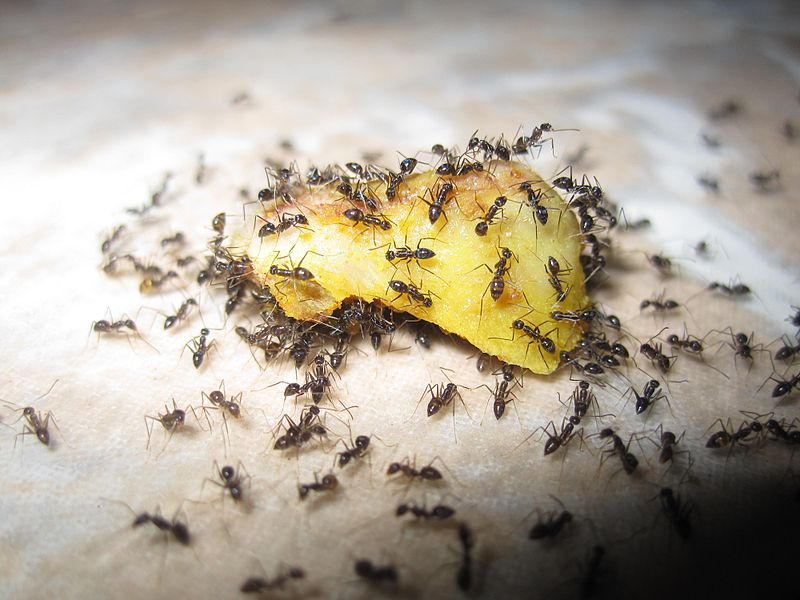
\includegraphics[width=4cm]{800px-Ants_eating_fruit}\vspace{1cm}}

\question{Why?}

\question{Computat{\redidot}onal Challenges\\
          \vspace{1cm}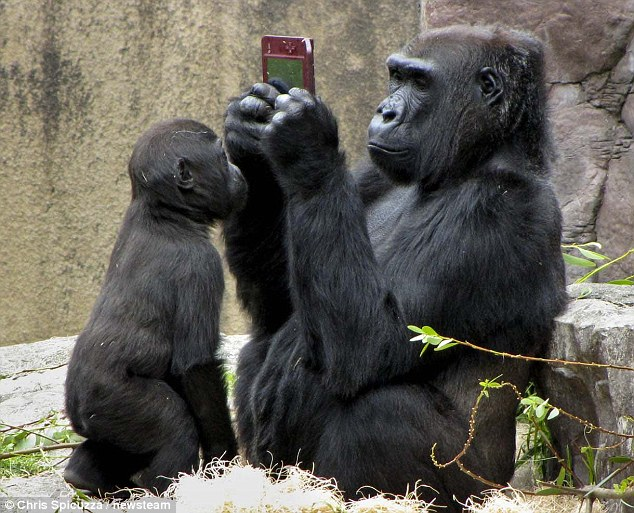
\includegraphics[width=4cm]{gorilla_tablet}}
\question{\red{Computat{\blackidot}onal} Challenges\\
          \vspace{1cm}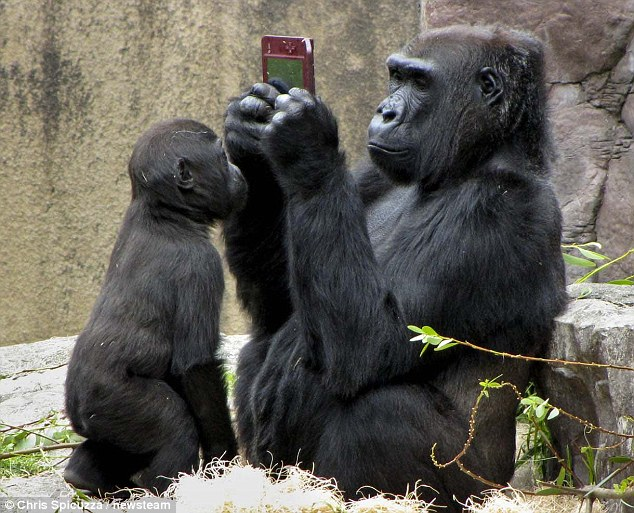
\includegraphics[width=4cm]{gorilla_tablet}}

\picw{Chinese-abacus}{}{1}{0}
%\pic{book_and_screen}{}
%\pic{8GB_vs_8Byte}{}

\frame{\frametitle{More and more diverse hardware}
 %\abspic{05_intel_ivy_bridge}         {-0.20}{0.0}{0.3}
 %\abspic{07_Nvidia_tesla_k10}         {-0.05}{0.4}{0.3}
 %\abspic{10_KnightsCornerChip_in_hand}{ 0.10}{0.7}{0.25}
 \abspic{arm}{-0.20}{0.0}{0.3}
 \abspic{icore9}{-0.25}{0.4}{.3}
 \abspic{radeon}{.15}{.1}{.3}
 \abspic{nvidia}{.10}{.4}{.3}
}
\picw{frontier}{}{1}{0}
%\picw{borg}{}{1}{0}

\frame{\frametitle{Computational Challenges}
 \abspic{640px-Gorilla_Scratching_Head}{0.2}{0.5}{0.35}
 \begin{itemize}
 \item Simulate cutting edge science
 \item Use latest numerical methods
 \item Make use of latest hardware
  \begin{itemize}
  \item Cache
  \pause
  \item Vector %(Kranc, NRPy)
  \pause
  \item Accelerators %(Kranc, NRPy)
  \pause
  \item Scale to many cores %(openmp)
  \pause
  \item Scale to many nodes %(MPI, Carpet)
  \pause
  \item Algorithms %(Adaptive Mesh Refinement, Carpet)
  %\item GPU %(AMReX?)
  %\item FPGA?
  %\item Q-Bits?
  %\item Neuromorphic chips?
  \end{itemize}
 \end{itemize}
}


\frame[containsverbatim]{ \frametitle{Computational Challenges}
  \begin{itemize}
    \item Efficient use of all hardware is complex and tedious.
    \item Requires experts from different disciplines
    \item Requires good data layouts and APIs 
    \item To ensure correctness, need good modularization on
          a number of levels
          and understanding of advanced programming concepts.
    \item Design and implementation needs to be carefully thought out
	  in order to ensure extensibility and portability.
  \end{itemize}
}

%\frame[containsverbatim]{ \frametitle{Domain Decomposition}
%  \begin{minipage}[b]{6.5cm}
%    \begin{itemize}
%      \item In a domain decomposition scheme, the discrete elements (points,
%            cells, particles, \ldots) are distributed among the processors.
%      \item Each process handles only those that it \emph{owns} (without
%            requiring communication).
%      \item Accessing elements from neighboring processes requires
%            communication (e.g.\ at domain boundaries).
%    \end{itemize}
%  \end{minipage}
%  \raisebox{2.0em}{
%    \begin{minipage}[t]{4.5cm}
%      \includegraphics[width=4.3cm]{pics/wire-frame}
%    \end{minipage}
%  }
%}

\frame { \frametitle{Domain Decomposition}
 Without Ghostzones:\\
 \begin{centering}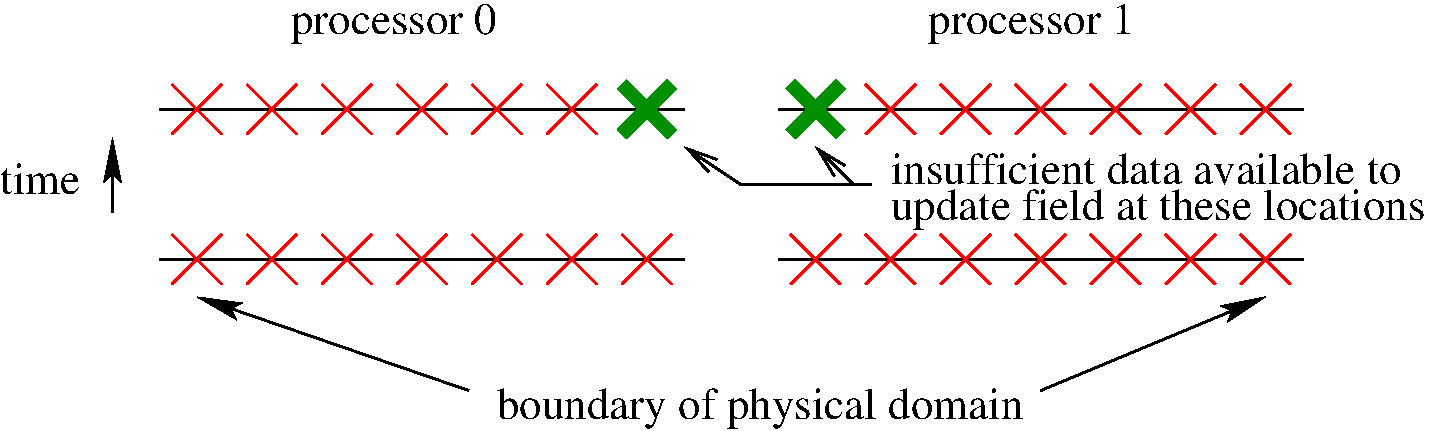
\includegraphics[width=9cm]{pics/1dnoghost}\\\end{centering}
 With Ghostzones:\\
 \begin{centering}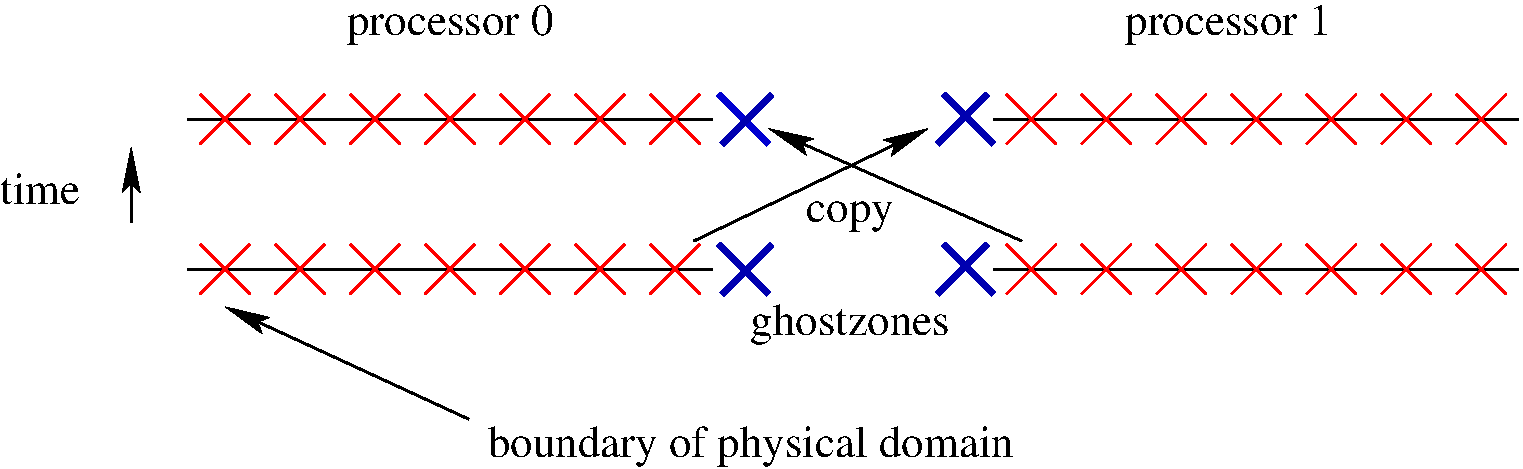
\includegraphics[width=9cm]{pics/withghost}\\\end{centering}
}

\frame { \frametitle{Domain decomposition}
 \begin{centering}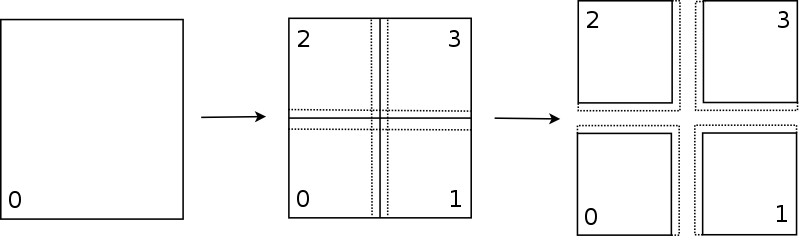
\includegraphics[width=11cm]{pics/domain_decomposition}\\\end{centering}
}
\frame { \frametitle{Multiblock and refinement}
 \begin{centering}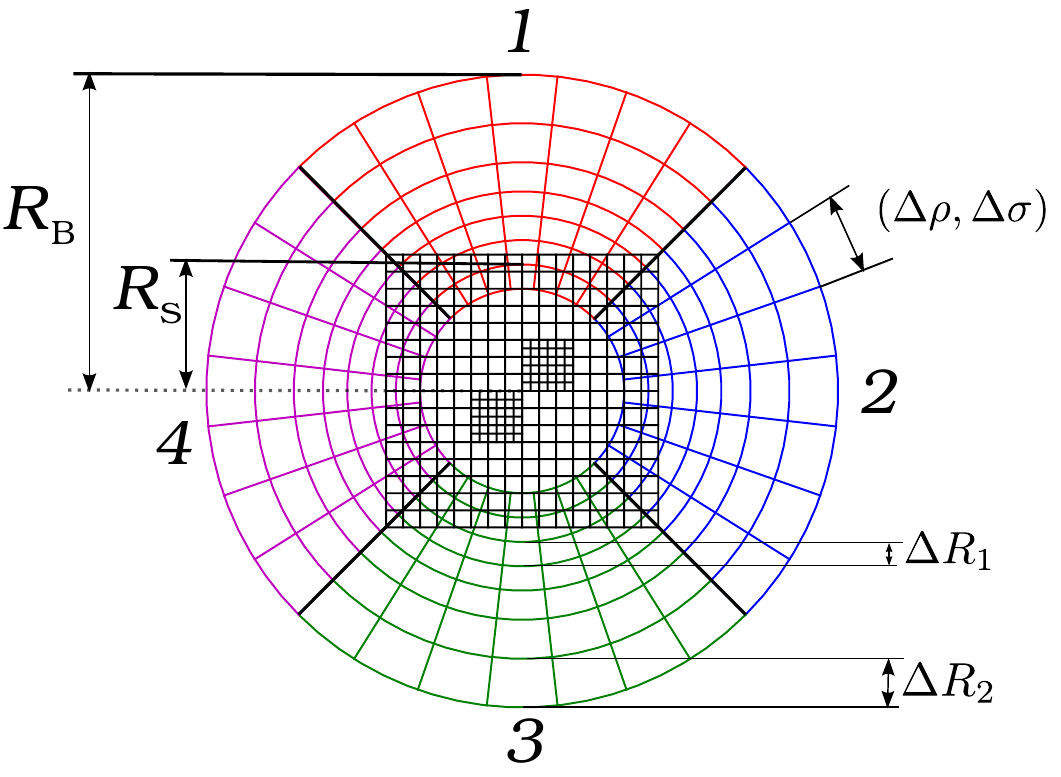
\includegraphics[width=11cm]{pics/multiblock}\\\end{centering}
}

\frame{\frametitle{Computational Challenges}
 \abspic{640px-Gorilla_Scratching_Head}{-0.1}{0.5}{0.35}
 \begin{itemize}
 \item Simulate cutting edge science
 \item Use latest numerical methods
 \item Make use of latest hardware
  \begin{itemize}
  %\item Cache
  \item Vector (Kranc, NRPy)
  \pause
  \item Scale to many cores (OpenMP)
  \pause
  \item Scale to many nodes (MPI, Carpet, CarpetX)
  \pause
  \item AMR (Adaptive Mesh Refinement, Carpet, CarpetX, MoL)
  \pause
  \item GPU (CarpetX)
  \pause
  \item Machine learning?
  \pause
  \item FPGA?
  \pause
  \item ASIC?
  \pause
  \item Neuromorphic processor?
  \pause
  \item Q-bits?
  \end{itemize}
 \end{itemize}
}

\frame{\frametitle{Computational Challenges}
 \abspic{640px-Gorilla_Scratching_Head}{-0.1}{0.5}{0.35}
More Mundane Challenges
\begin{itemize}
\pause
\item Efficient I/O
\pause
\item HDF5
\pause
\item Checkpoint/Restart
\pause
\item Parameter Parsing
\pause
\item Visualization
\pause
\item Analysis
\pause
\item Steering
\end{itemize}
}

%\frame[containsverbatim]{ \frametitle{The Wave Equation}
%  Approximating the pressure $P(x,t)$ with a grid function $P_i^{(n)}$.
%  \begin{minipage}[b]{3.05cm}
%    \includegraphics[width=3cm]{pics/discretisation}
%  \end{minipage}
%  \raisebox{8em}{
%  \begin{minipage}[t]{8.5cm}
%    \begin{eqnarray}
%      \frac{\partial^2 P}{\partial t^2} & = & 
%       v^2\frac{\partial^2 P}{\partial x^2} \nonumber \\
%      & \Downarrow & \nonumber \\
%      \frac{P_i^{(n+1)}-2 P_i^{(n)}+P_i^{(n-1)}}{\Delta t^2} & = &
%      v^2\frac{P_{i+1}^{(n)}-2 P_i^{(n)}+P_{i-1}^{(n)}}{\Delta x^2} \nonumber
%    \end{eqnarray}
%  \end{minipage}}
%  The error from this time and space discretisation is $O(h^2)$.
%}

\question{Collaborat{\redidot}ve Challenges\\
          \vspace{1cm}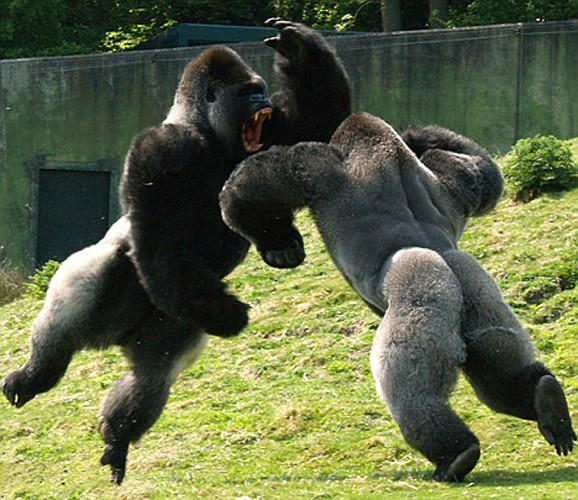
\includegraphics[width=4cm]{gorilla_fight}}
\question{\red{Collaborat{\blackidot}ve} Challenges\\
          \vspace{1cm}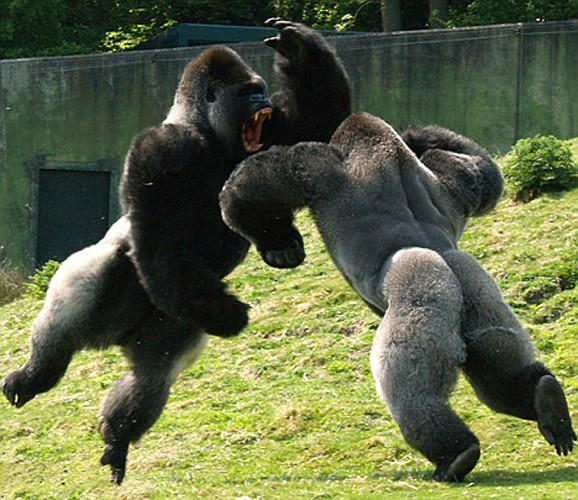
\includegraphics[width=4cm]{gorilla_fight}}

\frame{
  \abspic{community_only_problem}    {-0.1}{0.1}{0.6}
}

\frame{
  \abspic{community_with_problem}    {-0.1}{0.1}{0.6}
  \abspic{hurricane}     {-0.35}{0.05}{0.2}
  \abspic{wind_park}     {-0.30}{0.73}{0.2}
  \abspic{space_shuttle} { 0.20}{0.00}{0.2}
  \abspic{crab}          { 0.20}{0.75}{0.2}
}

\frame{
  \abspic{community_with_computation}{-0.1}{0.1}{0.6}
  \abspic{hurricane}     {-0.35}{0.05}{0.2}
  \abspic{wind_park}     {-0.30}{0.73}{0.2}
  \abspic{space_shuttle} { 0.20}{0.00}{0.2}
  \abspic{crab}          { 0.20}{0.75}{0.2}
  \abspic{bluewaters}        {-0.07}{0.40}{0.15}
  \abspic{tianhe1}       { 0.31}{0.40}{0.15}
}

\frame{
  \abspic{community_of_groups}       {-0.1}{0.1}{0.6}
  \abspic{hurricane}     {-0.35}{0.05}{0.2}
  \abspic{wind_park}     {-0.30}{0.73}{0.2}
  \abspic{space_shuttle} { 0.20}{0.00}{0.2}
  \abspic{crab}          { 0.20}{0.75}{0.2}
  \abspic{bluewaters}        {-0.07}{0.40}{0.15}
  \abspic{tianhe1}       { 0.31}{0.40}{0.15}
}

\frame{
  \abspic{community_of_groups}       {-0.1}{0.1}{0.6}
  \abspic{hurricane}     {-0.35}{0.05}{0.2}
  \abspic{wind_park}     {-0.30}{0.73}{0.2}
  \abspic{space_shuttle} { 0.20}{0.00}{0.2}
  \abspic{crab}          { 0.20}{0.75}{0.2}
  \abspic{email}         { 0.06}{0.38}{0.10}
  \abspic{phone}         { 0.04}{0.53}{0.10}
  \abspic{irc}           { 0.25}{0.40}{0.10}
  \abspic{www}           { 0.25}{0.55}{0.10}
}

\frame{
  \abspic{email}         { 0.06}{0.38}{0.10}
  \abspic{phone}         { 0.04}{0.53}{0.10}
  \abspic{irc}           { 0.25}{0.40}{0.10}
  \abspic{www}           { 0.25}{0.55}{0.10}
  \pause
  \abspic{Subversion-logo}{-0.28}{0.20}{0.23}
  \abspic{Git-logo}       {-0.20}{0.40}{0.13}
  \abspic{Mercurial_logo} {-0.20}{0.70}{0.13}
  \pause
  \abspic{github_logo}    { 0.10}{0.05}{0.10}
  \pause
  \abspic{Mediawiki_logo} { 0.10}{0.70}{0.15}
  \pause
  \abspic{Workshop}       { 0.35}{0.10}{0.05}
}

\frame{
  \abspic{community_with_problems}   {-0.1}{0.1}{0.6}
  \abspic{hurricane}     {-0.35}{0.05}{0.2}
  \abspic{wind_park}     {-0.30}{0.73}{0.2}
  \abspic{space_shuttle} { 0.20}{0.00}{0.2}
  \abspic{crab}          { 0.20}{0.75}{0.2}
}

\frame{
  \abspic{community_with_competition}{-0.1}{0.1}{0.6}
  \abspic{crab}          {-0.35}{0.05}{0.2}
  \abspic{crab}          {-0.30}{0.73}{0.2}
  \abspic{crab}          { 0.20}{0.00}{0.2}
  \abspic{crab}          { 0.20}{0.75}{0.2}
}

\frame{
  \abspic{community_with_standards}{-0.1}{0.1}{0.6}
  \abspic{hurricane}     {-0.35}{0.05}{0.2}
  \abspic{wind_park}     {-0.30}{0.73}{0.2}
  \abspic{space_shuttle} { 0.20}{0.00}{0.2}
  \abspic{crab}          { 0.20}{0.75}{0.2}
}

\frame{
  \abspic{community_with_standards}{-0.1}{0.1}{0.6}
  \abspic{hurricane}     {-0.35}{0.05}{0.2}
  \abspic{wind_park}     {-0.30}{0.73}{0.2}
  \abspic{space_shuttle} { 0.20}{0.00}{0.2}
  \abspic{crab}          { 0.20}{0.75}{0.2}
  \abspic{Imperial-Metric}{0.35}{0.40}{0.12}
  \pause
  \abspic{hdf_logo}      {-0.10}{0.45}{0.1}
}

\frame{
  \abspic{community_with_tools}{-0.1}{0.1}{0.6}
  \abspic{hurricane}     {-0.35}{0.05}{0.2}
  \abspic{wind_park}     {-0.30}{0.73}{0.2}
  \abspic{space_shuttle} { 0.20}{0.00}{0.2}
  \abspic{crab}          { 0.20}{0.75}{0.2}
}
\frame{
  \abspic{community_with_tools_examples}{-0.1}{0.1}{0.6}
}
\frame{
  \abspic{community_with_tools_examples}{-0.1}{0.1}{0.6}
  \abspic{Tux-linux_logo}     {-0.35}{0.05}{0.2}
  \abspic{Windows_logo}       {-0.30}{0.73}{0.2}
  \abspic{Apple_Logo}         { 0.20}{0.03}{0.15}
  \abspic{Tux-linux_logo}     { 0.17}{0.13}{0.2}
  \abspic{Apple_Logo}         { 0.24}{0.77}{0.15}
}

\frame{
  \abspic{community_with_credit}{-0.1}{0.1}{0.6}
  \abspic{hurricane}     {-0.35}{0.05}{0.2}
  \abspic{wind_park}     {-0.30}{0.73}{0.2}
  \abspic{space_shuttle} { 0.20}{0.00}{0.2}
  \abspic{crab}          { 0.20}{0.75}{0.2}
}
\frame{
  \abspic{community_with_credit}{-0.1}{0.1}{0.6}
  \abspic{crab}          {-0.35}{0.05}{0.2}
  \abspic{crab}          {-0.30}{0.73}{0.2}
  \abspic{crab}          { 0.20}{0.00}{0.2}
  \abspic{crab}          { 0.20}{0.75}{0.2}
}


\frame{\frametitle{Collaborative Challenges}
 \abspic{germany}              {-0.10}{0.42}{0.2}
 \abspic{germany_map}          { 0.12}{0.52}{0.2}
 \abspic{800px-Los_Angeles_Skyline_telephoto}{-0.05}{0.68}{0.2}
 \abspic{georgia}              { 0.26}{0.65}{0.18}
 \abspic{ncsa}                 { 0.42}{0.55}{0.21}
 \abspic{neworleans}           { 0.55}{0.65}{0.18}
How can we work together?
\begin{itemize}
    \item Researchers in the USA
    \begin{itemize}
    \begin{minipage}[t]{5cm}
    \begin{multicols}{2}
        \item Arizona
        \item Florida
        \item Georgia
        \item Louisiana
        \item Illinois
        \item Indiana
        \item New York
        \item Idaho
        \item Tenessee
        \item Texas
        \item Pennsylvania
        \item California
    \end{multicols}
    \end{minipage}
    \end{itemize}
    \item In other countries
    \begin{itemize}
    \begin{minipage}[t]{5cm}
    \begin{multicols}{2}
        \item Canada
        \item France
        \item Germany
        \item Ireland
        \item Italy
        \item Mexico
        \item Netherlands
        \item Portugal
        \item Spain
        \item Turkey
        \item United Kingdom
        \item and many more
    \end{multicols}
    \end{minipage}
    \end{itemize}
\end{itemize}
}

\frame{\frametitle{Einstein Toolkit}
 \abspic{einstein}{-0.2}{0.6}{0.23}
 \abspic{cactuslogo}{0.28}{0.20}{.11}
 \abspic{simfac-trim}{0.31}{0.32}{.15}
 \abspic{kranc-trim}{0.45}{0.20}{.11}
 \abspic{Nerpy}{0.56}{0.30}{.15}
\begin{columns}
\begin{column}{0.5\textwidth}
Goals:
\begin{itemize}
\item Community Driven
\item Core computational tool for numerical astrophyscis
\item General purpose tool!
\end{itemize}
Components:
\begin{itemize}
\item Cactus
\item Simulation Factory
\item Kranc
\item NRPy
\item Science Modules
\end{itemize}
\end{column}
\begin{column}{0.5\textwidth}
Guiding Principles
\begin{itemize}
\item Open
\item Community Driven
\item Good interfaces
\item Separation of physics
      from computational
      infrastructure
\item Production ready
\item High quality code
\end{itemize}
\end{column}
\end{columns}
}

\frame{\frametitle{Einstein Toolkit as growing project}
 \abspic{jigsaw1} {-0.082}{0.35}{0.16}
 \vspace{-4cm}
 \begin{itemize}
  \item \small Initially: some infrastructure, some application code
 \end{itemize}
}
\frame{\frametitle{Einstein Toolkit as growing project}
 \abspic{jigsaw2} {-0.2}{0.2}{0.4}
 \vspace{-4cm}
 \begin{itemize}
  \item \small Growing application suite
 \end{itemize}
}
\frame{\frametitle{Einstein Toolkit as growing project}
 \abspic{jigsaw3} {-0.2}{0.14}{0.52}
 \vspace{-4cm}
 \begin{itemize}
  \item \small Growing infrastructure ``return''
 \end{itemize}
}
\frame{\frametitle{Einstein Toolkit as growing project}
 \abspic{jigsaw4} {-0.205}{0.135}{0.525}
 \vspace{-4cm}
 \begin{itemize}
  \item \small Users from more fields of science
 \end{itemize}
}
\frame{\frametitle{Einstein Toolkit as growing project}
 \abspic{jigsaw5} {-0.205}{0.135}{0.525}
 \vspace{-4cm}
 \begin{itemize}
  \item \small Most modules open-source, but not necessarily all
 \end{itemize}
}

\question{Base Modules\\*[1em]
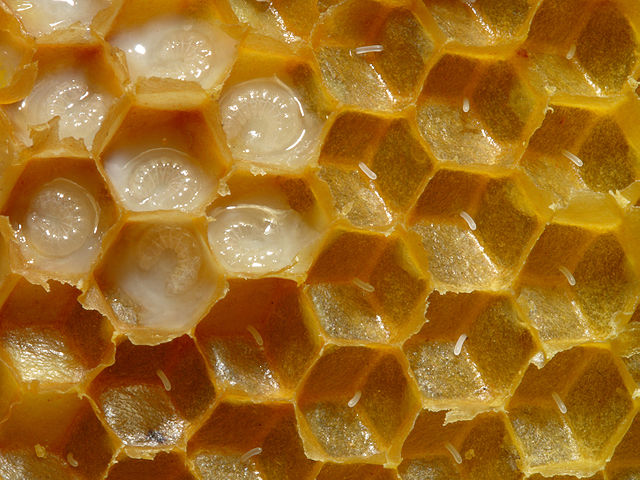
\includegraphics[width=0.4\textwidth]{640px-Bienenwabe_mit_Eiern_und_Brut_5}}

\frame{\frametitle{The Einstein Equations}
  \abspic{Eeq_Eeq}{-0.25}{0.0}{0.70}
}
\frame{
  \abspic{Eeq_curvature}{-0.25}{0.0}{0.70}
}
\frame{
  \abspic{Eeq_constants}{-0.25}{0.0}{0.70}
}
\frame{
  \abspic{Eeq_matter}{-0.25}{0.0}{0.70}
}
\frame{
  \abspic{Eeq_all}{-0.25}{0.0}{0.70}
}

\frame{
  \abspic{ET_layout_Eeq}{-0.25}{0.0}{0.70}
}
\frame{
  \abspic{ET_layout_ADMBase}{-0.25}{0.0}{0.70}
}
\frame{
  \abspic{ET_layout_Base2}{-0.25}{0.0}{0.70}
}
\frame{
  \abspic{ET_layout_Tmunu}{-0.25}{0.0}{0.70}
}
\frame{
  \abspic{ET_layout_evolution}{-0.25}{0.0}{0.70}
}
\frame{
  \abspic{ET_layout_all}{-0.25}{0.0}{0.70}
}
\frame{
  \abspic{ET_layout_multiple}{-0.25}{0.0}{0.70}
}

\frame{\frametitle{Guiding Principles}
 \abspic{opensource_logo}{0.2}{0.7}{0.2}
 \begin{itemize}
  \item Open, community-driven software development
  \item Separation of \textbf{physics} software and \textbf{computational} infrastructure
  \item Stable interfaces, allowing extensions
  \item Simplify usage where possible:
   \begin{itemize}
    \item Doing science $>>$ Running a simulation
    \item Students need to know a lot about physics\\
           (meaningful initial conditions, numerical stability,\\
           accuracy/resolution, have patience, have curiosity,\\
           develop a ``gut feeling'' for what is right ...)
    \item Einstein Toolkit \textbf{cannot} give that, \textbf{however}:\\
          Open codes that are easy to use allow to concentrate on these things!
   \end{itemize}
 \end{itemize}
}

\frame{\frametitle{Credits, Citations}
 \abspic{barretr_Book.png}{0.2}{0.7}{0.2}
 In academics: citations, citations, citations!\\
 For Einstein Toolkit:
 \begin{itemize}
  \item Open and free source
  \item No \textbf{requirement} to cite anything
  \item However: \textbf{requested} to cite 
  \begin{itemize}
   \item The DOI doi:10.5281/zenodo.3350841
   \item Maybe the ET or Cactus papers
   \item Some papers for the components list a few as well
   \item List published on website and manage through publication database
  \end{itemize}
  \item Soon: auto-generate list of citations during simulation run
 \end{itemize}
}

\section{Vision}
\frame{\frametitle{Vision}
 \abspic{arrow}{0}{0.65}{0.18}
 Cutting Edge / Future
 \begin{itemize}
  %\item Inclusion of ``more physics'', e.g. general \\MHD, tabulated equations of state
  %\item Improve scaling of existing mesh methods
  \item New Driver Thorn: CarpetX (Meitner Release)
  \item New Hydro Thorn: AsterX (Next Release?)
  \item New Boundary Thorn: NewRadX (Landau Release)
  %\item New Spherical Coordinates Thorn (RIT)
  \item GRHayL thorns (Meitner, Landau, etc...)
  \item Python Code Generator: Full thorn output from NRPy
  \item Kerr background support in SelfForce1D (Soon?)
 \end{itemize}
% Recent
% \begin{itemize}
%  \item CarpetX was added
%  \item GRHayL: General Relativistic Hydrodynamics Library
%  \item DNSdata for importing SGRID initial data
%%  \item Seed\_Magnetic\_Fields
%  %\item PN based initial data and eccentricity reduction
%  %\item New Declarative Synchronization: Presync
%  %\item Python based simulation analysis: kuibit
% \end{itemize}
}

\section{Summary}
\frame{\frametitle{Summary}
 \abspic{people}    {-0.15}{0.55}{0.15}
 \abspic{opensource_logo}{0.05}{0.8}{0.1}
 \begin{centering}
  \href{run:mplayer -noaspect -fs -zoom -vo xv ../pics/Einstein_Toolkit.avi}{
    
\includegraphics[height=2cm]{cactuslogo}}\\
 \end{centering}
 {\large Einstein Toolkit\\}
 \begin{itemize}
  \item http://www.einsteintoolkit.org/
  \item Tools for high-performance computing in numerical relativity
  \item Open Source
  \item World-wide, open Community
  \item Used in high-end research
 \end{itemize}
}

\frame{\frametitle{Supported By}
The Einstein Toolkit is supported by \\
NSF 2004157/2004044/2004311/2004879/2003893,
NSF 1550551/1550461/1550436/1550514
Any opinions, findings, and conclusions or recommendations expressed in this material are those of the author(s) and do not necessarily reflect the views of the National Science Foundation.
}


\end{document}

